\chapter{Codes correcteurs d'erreurs et Algèbre de Boole}
\section{Code}
Pour pouvoir, en binaire, représenter les chiffres de 0 à 9, il nous faut au minimum 4 bits ($\log_2 10$). Donc, nous perdons 6 codes du à l'arrondissement à 4 bits (1010, 1011, 1100, 1101, 1101 et 1111). En octal et hexadécimal, c'est plus pratique car il n'y a pas de perte du à l'arrondissement ($\log_2 8=3$ et $\log_2 16=4$).Il y a donc, d'autres façons de coder en fonction de l'utilisation qu'on en fait. On en distingue 3 classes: 
\begin{enumerate}
	\item 	Codes pondérés (\textit{weighted codes})
	\begin{itemize}
		\item 8421 \textit{Binary coded Decimal} (BCD) où chaque chiffre est codé séparément
		\item Codes auto-complémentaires
		\begin{itemize}
			\item 2421 Code
			\item Code excédent 3 (Excess 3)
		\end{itemize}
	\end{itemize}
	\item Codes non-pondérés
	\begin{itemize}
		\item Code Gray (code cyclique)
		\item \textit{American Standard Code for Information Interchage} (code ASCII)
	\end{itemize}
	\item Code détecteurs d'erreur
\end{enumerate}
\subsection{Codes pondérés}
Voici une table pour bien comprendre comment fonctionnent les codes auto-complémentaires (le $-$ de $-3$ correspond au chiffre négatif)
\begin{table}[H]
	\centering
	\begin{tabular}{c|c|c|c}
		Décimal & 8421 (BCD) & 2421 & 642-3 \\
		\hline
		0 & 0000 & 0000 & 0000\\
		\hline
		1 & 0001 & 0001 & 0101\\
		\hline
		2 & 0010 & 0010 & 0010\\
		\hline
		3 & 0011 & 0011 & 1001\\
		\hline
		4 & 0100 & 0100 & 0100\\
		\hline
		5 & 0101 & 1011 & 1011\\
		\hline
		6 & 0110 & 1100 & 0110\\
		\hline
		7 & 0111 & 1101 & 1101\\
		\hline
		8 & 1000 & 1110 & 1010\\
		\hline
		9 & 1001 & 1111 & 1111		
	\end{tabular}
	\caption{Code auto-complémentaire}
\end{table}
\subsubsection{Addition en BCD}
L'addition en BCD est simple, on additionne par 4 bits (chaque chiffre composant la base 10). Si le chiffre est $\geq 10$ (i.e. $1010$), on ajoute $+6\,(0110)_2$ car cela correspond à un report de 10 en binaire. En effet, regroupé par 4 correspond à de l'hexadécimal, du coup, pour passer de 10 à 0, il faut ajouter 6 ($A\overset{+1}{\rightarrow}B\overset{+1}{\rightarrow}\dots\overset{+1}{\rightarrow}F\overset{+1}{\rightarrow}0$). Exemple:
\begin{table}[H]
	\centering
	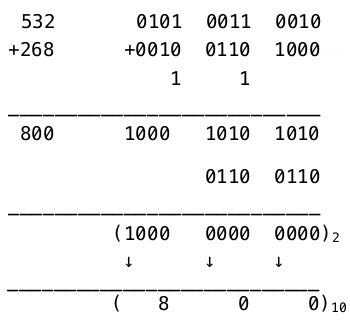
\includegraphics[scale=0.5]{ch2/image1}
\end{table}
\subsection{Codes non-pondérés}
\subsubsection{Code Gray}
Le code Gray est un code suivant le principe de \textit{Look-up Table}, c'est-à-dire que la conversion ne suit pas une règle mais une table de correspondance associant des valeurs. Le principe du Gray est que 2 codes voisins ne diffèrent que par la valeur d'un bit.
\begin{table}[H]
	\centering
	\begin{tabular}{c|c}
		Décimal & Gray \\
		\hline
		0 & 000\\
		 \hline
		1 & 001\\
		 \hline
		2 & 011\\
		 \hline
		3 & 010\\
		 \hline
		4 & 110\\
		 \hline
		5 & 111\\
		 \hline
		6 & 101\\
		 \hline
		7 & 101		 
	\end{tabular}
	\caption{Code Gray}
\end{table}
\subsubsection{Code ASCII}
Le code ASCII est utilisé pour coder les caractères dans des systèmes de traitement numérique, comme les majuscules, les signes de ponctuation, et cetera. Le code est basé sur 8 bits, donc 256 possibilités, mais en réalité, on en utilise que 128.
\begin{figure}[H]
	\centering
	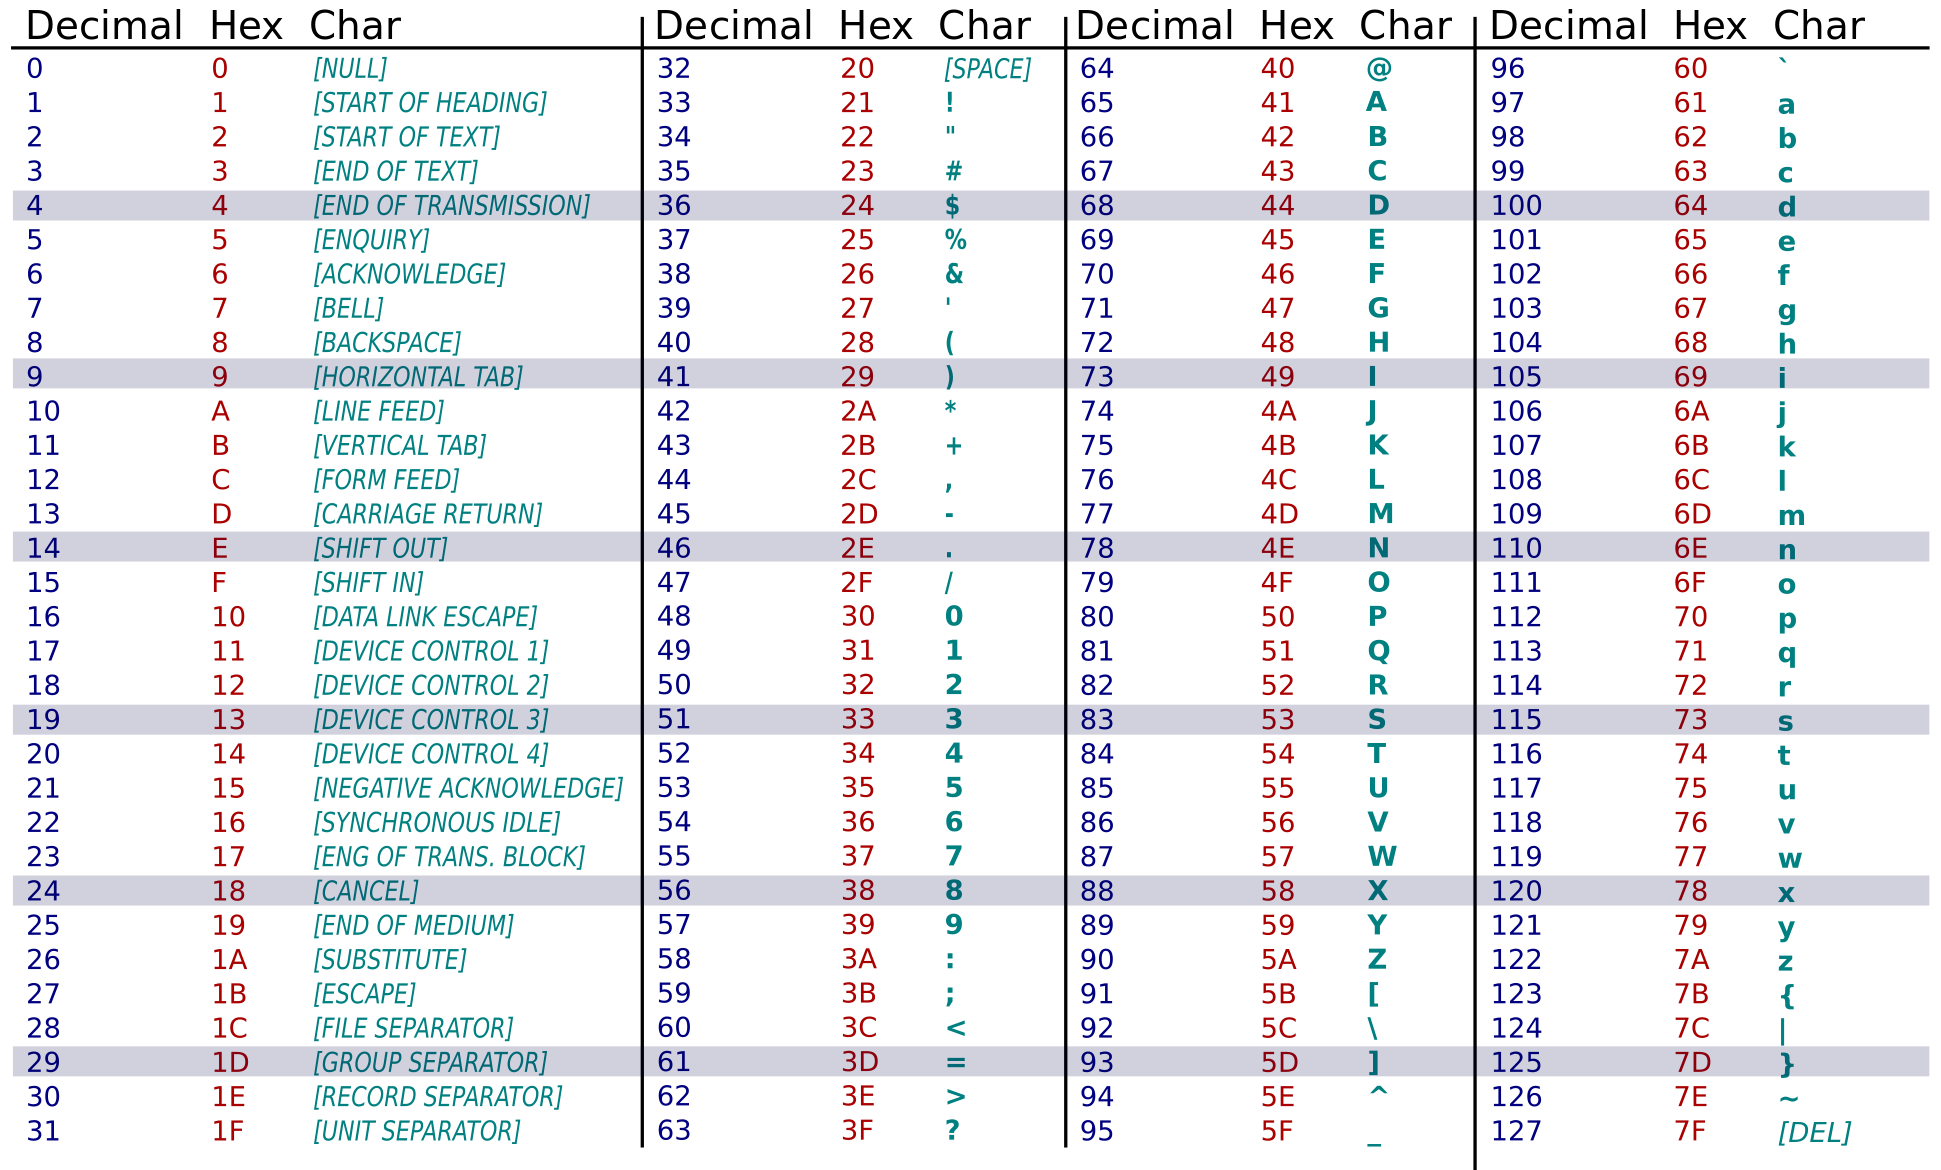
\includegraphics[width=\textwidth]{ch2/image2}
	\caption{Table ASCII}
\end{figure}
\subsection{Codes correcteurs}
\paragraph{Distance de Hamming} quantifie la distance (la différence) entre 2 séquences de symboles (ex : $d(0111,1010)=3$).
\paragraph{n-cube} cube à n dimensions ($2^n$ sommets) où chaque n-bit string est représenté par un des sommets. \textbf{Les sommets adjacents ont une distance de Hamming de 1}.
\begin{figure}[H]
	\centering
	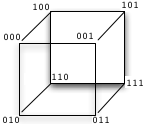
\includegraphics[scale=0.6]{ch2/image3}
	\caption{n-cube pour $n=3$}
\end{figure}
\subsubsection{Principe général}
Sur n-bits, on peut coder $2^n$ mots différents, si on rajoute 1 bit, nous avons $2^n$ mots supplémentaires. Nous pouvons donc grâce à cela, définir n mots qualifié d'erronés, ce qui sera utile pour détecter les erreurs (comme des erreurs de transmission).
\subsubsection{Codes de parité paire ou impaire (\textit{even (odd) parity codes})}
On code les mots de n-bits sur $(n+1)$ bits, ainsi nous avons autant de mots corrects que d'erronés. Le critère de correction est défini par le $(n+1)$\up{ème} bit.\\

Il faut compter le nombre de \textbf{1} et suivre la convention définie. Les 2 conventions sont: 
\begin{itemize}
	\item Bit de parité paire: 1 si c'est un nombre \textbf{impair}
	\item Bit de parité impair: 1 si c'est un nombre \textbf{pair}
\end{itemize}
Lors du calcul de parité, on peut ou non tenir compte du bit de parité (le $(n+1)$\up{ème}). Ici, on en tiendra pas compte.\\

Ce qui est intéressant, c'est de rajouter un bit de parité pour chaque poids (pour m-mots de n-bits, nous aurions donc des mots de $n+1$ pour le bit de parité et $m+1$ mot pour le bit de parité de poids). Ainsi, nous pourrions déterminer exactement le bit qui est erroné.
\begin{figure}[H]

	\begin{minipage}{0.55\textwidth}
	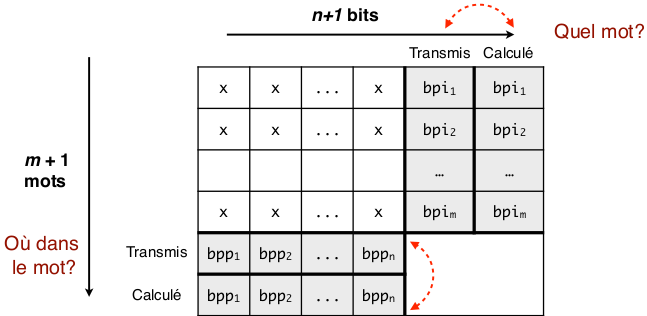
\includegraphics[scale=0.4]{ch2/image4}
	\end{minipage}
	\begin{minipage}{0.5\textwidth}
		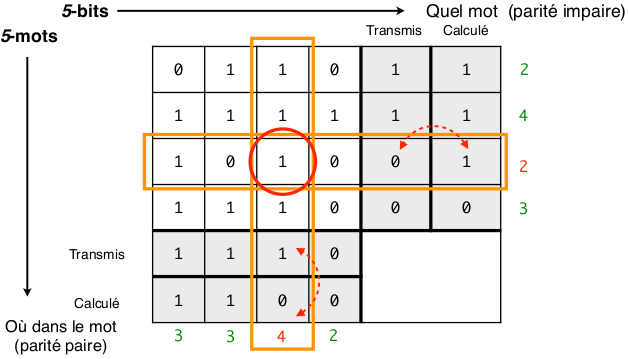
\includegraphics[scale=0.4]{ch2/image5}
	\end{minipage}
\end{figure}

\section{Algèbre de Boole}
\subsection{Définition}
Algèbre de Boole est un quadruplet $\{B,',\cdot,+\}$ où
$\left\{
\begin{array}{l l}
	B & \text{est un ensemble de 2 valeurs}\\
	' & \text{est l'opérateur de complément (parfois symbole \ $\bar{ }$ )}\\
	\cdot & \text{est l'opérateur \textbf{et}}\\
	+ & \text{est l'opérateur \textbf{ou}}
\end{array}\right.$\\\\
En fonction des définitions des opérateurs, on peut définir plusieurs algèbre de Boole. On ne s'intéressera ici que de celle-ci pour 2 valeurs.
\subsection{Algèbre de Boole à 2 valeurs}
\subsubsection{Définition}
L'algèbre de Boole à 2 valeurs est défini par (introduite par \textsc{Shannon}):
\begin{itemize}
	\item[$B=$]$\{0,1\}$
	\begin{itemize}
		\item[$0$]= faux
		\item[$1$]= vrai
	\end{itemize}
	\item[$+$]= ou inclusif (or)
	\item[$\cdot$]= et (and)
\end{itemize}
Les opérateurs $+$ et $\cdot$ peuvent être définis par \textbf{Tables de Vérités} (\textit{TdV}) suivantes:
\begin{table}[H]
	\begin{minipage}{0.5\textwidth}
		\centering
	$\begin{array}{c|c|c}
		x & y &  x\cdot y\\
		\hline
		0 & 0 & 0\\
		0 & 1 & 0\\
		1 & 0 & 0\\
		1 & 1 & 1
	\end{array}$
	\end{minipage}
	\begin{minipage}{0.5\textwidth}
		\centering
		$\begin{array}{c|c|c}
		x & y &  x+y\\
		\hline
		0 & 0 & 0\\
		0 & 1 & 1\\
		1 & 0 & 1\\
		1 & 1 & 1
		\end{array}$
	\end{minipage}
\end{table}
Le nombre de variables ($=a$) détermine le nombre de lignes de la TdV ($2^a$). On remarque entre autre une petite propriété des TdV sur la valeur de chaque variable. Le LSD (ici y), se définit comme : $0,1,0,1,\dots$ ensuite (ici $x$) : $00,11,00,11,\dots$ et encore après $0000,1111,0000,\dots$ Donc chaque variable répète sa valeur $2^n$ fois où $n=$ poids de chaque variable.
\subsubsection{Axiomes}
E. V. \textsc{Huntigton} posa 6 axiomes pour le cas de l'algèbre de Boole à 2 valeurs $B=\{0,1\}$. Ces axiomes sont vérifiables par \textit{TdV}. Les axiomes sont:
\begin{itemize}
	\item[-- Axiome 1.] $B$ est \textbf{fermé} pour $+$ et pour $\cdot$
	\begin{table}[H]
		\begin{minipage}{0.3\textwidth}
			\centering
			$\begin{array}{c|c}
				x & x'\\
				\hline
				0 & 1\\
				1 & 0
			\end{array}$
		\end{minipage}
		\begin{minipage}{0.3\textwidth}
			\centering
			$\begin{array}{c|c|c}
				x & y &x\cdot y\\
				\hline
				0 & 0 & 0\\
				0 & 1 & 0\\
				1 & 0 & 0\\
				1 & 1 & 1
			\end{array}$
		\end{minipage}
		\begin{minipage}{0.3\textwidth}
			\centering
			$\begin{array}{c|c|c}
				x & y &x+ y\\
				\hline
				0 & 0 & 0\\
				0 & 1 & 1\\
				1 & 0 & 1\\
				1 & 1 & 1
			\end{array}$
		\end{minipage}
	\end{table}
	\item[-- Axiome 2.] $B$ a un \textbf{neutre} pour $+$ (noté $0$) et pour $\cdot$ (noté $1$)
	\begin{equation}
		\begin{array}{l}
			0+0=0\\
			1+0=1
		\end{array}
		\quad\text{et}\quad 
		\begin{array}{c}
			0\cdot 1=0\\
			1\cdot 1=1
		\end{array}
	\end{equation}
	\item[-- Axiome 3.] $B$ est \textbf{commutatif} par rapport à $+$ et $\cdot$
	\begin{equation}
		x+y=y+x\quad\text{et}\quad x\cdot y=y\cdot x
	\end{equation}
	\item[-- Axiome 4.] $\cdot$ \textbf{distribue} $+$ et $+$ distribue $\cdot$
	\begin{equation}
		x\cdot(y+z)=x\cdot y+x\cdot z\quad\text{et}\quad x+(y\cdot z)=(x+y)\cdot(x+z)
	\end{equation} 
	\hfill Preuve par TdV
	\item[-- Axiome 5.] $\exists$ \textbf{complément} de x (noté $x'$, $\bar{x}$ ou not($x$))
	\item[-- Axiome 6.] Il y a au moins 2 éléments $x,y$ du $B$ tels que $x\neq y$
\end{itemize}
\subsubsection{Théorèmes}
À partir de ces axiomes, nous pouvons définir les théorèmes suivant (à droite, les théorèmes issus du \nameref{subsubsec : dualité}):
\begin{multicols}{2}
	\textbf{Normaux}
\begin{itemize}
	\item[-- Théorème 1.] Indempotence pour $+$ et $\cdot$
	\begin{equation}
		x+x=x\quad\text{et}\quad x\cdot x=x
	\end{equation}
	\item[-- Théorème 2.]
	\begin{equation}
		x+1=1\quad\text{et}\quad x\cdot 0=0
	\end{equation}
	\item[-- Théorème 3.] Absorption
	\begin{equation}
		x\cdot(x+y)=x
	\end{equation}
	\item[-- Théorème 4.] Involution
	\begin{equation}
		(x')'=x
	\end{equation}
	\item[-- Théorème 5.] Associativité
	\begin{equation}
		\begin{split}
			(x+y)+z&=x+(y+z)\\&\text{et}\\(x\cdot y)\cdot z&=x\cdot (y\cdot z)
		\end{split}
	\end{equation}
	\item[-- Théorème 6.] Lois de \textsc{De Morgan}
	\begin{equation}
		\begin{split}
			(x+y)'&=x'\cdot y'\\&\text{et}\\ (x\cdot y)'&=x'+y'
		\end{split}
	\end{equation}
	\item[-- Théorème 7.] Consensus
	\begin{equation}
		x\cdot y+x'\cdot z+y\cdot z = x\cdot y + x'\cdot z
	\end{equation}
\end{itemize}
\columnbreak
 \textbf{Duaux} 
 \begin{itemize}
 	\item[-- Théorème 1.] Indempotence pour $+$ et $\cdot$
 	\begin{equation}
	 	 x\cdot x=x\quad\text{et}\quad x+x=x
 	\end{equation}
 	\item[-- Théorème 2.]
 	\begin{equation}
 		x\cdot 0=0\quad\text{et}\quad x+1=1
 	\end{equation}
 	\item[-- Théorème 3.] Absorption
 	\begin{equation}
 		x+(x\cdot y)=x
 	\end{equation}
 	\item[-- Théorème 4.] Involution
 	\begin{equation}
 		(x')'=x
 	\end{equation}
 	\item[-- Théorème 5.] Associativité
 	\begin{equation}
	 	\begin{split}
		 	(x\cdot y)\cdot z&=x\cdot (y\cdot z)\\&\text{et}\\(x+ y)+ z&=x+(y+ z)
	 	\end{split}
 	\end{equation}
 	\item[-- Théorème 6.] Lois de \textsc{De Morgan}
 	\begin{equation}
	 	\begin{split}
		 	(x\cdot y)'&=x'+y'\\&\text{et}\\(x+y)'&=x'\cdot y' 
	 	\end{split}
 	\end{equation}
 	\item[-- Théorème 7.] Consensus
 	\begin{equation}
 	(x+y)\cdot (x'+ z)\cdot(y+ z) = (x+ y) \cdot (x'+ z)
 	\end{equation}
 \end{itemize}
\end{multicols}
\danger Consensus (et son dual) pas évident (et utile)
\subsubsection{Principe de dualité}
\label{subsubsec : dualité}
Dans l'algèbre de Boole, tout résultat peut se présenter sous 2 formes dites duales.\\
Soit $S$ un résultat, son dual $S^*$ est obtenu en \textbf{permutant} :
\begin{itemize}
	\item les opérateurs $+$ et $\cdot$
	\item les symboles $0$ et $1$ de $B$
\end{itemize}
\textbf{
	\begin{center}
		Si un résultat $S$ est vrai dans l'algèbre de Boole,\\il en est de même pour son dual $S^*$
	\end{center}
}
Nous pouvons bien évidement généraliser ce principe pour une expression Booléenne à $n$-variables
\section{Fonctions logiques}
\paragraph{Entrées} arguments d'une fonction logique
\paragraph{Sorties} évaluation de(s) la(es) fonction(s)\\

Chaque sortie aura une fonction logique qui lui est propre
\subsection{Représentation des fonctions logiques}
Il y a différentes formes pour représenter des fonctions logiques :
\begin{itemize}
	\item \textbf{Fonctions logiques}: représentation compacte pour un faible nombre de variables. Pratique pour une manipulation manuelle ou «crayon et papier».
	\item \textbf{Tables de Vérité}: représentation tabulaire, proche de la représentation de type mémoire numérique (style \textit{Look-up-Table}).
	\item \textbf{Schématique}: représentation graphique ; proche du monde de la réalisation physique ; facile à comprendre (mais peut être très compliqué pour un grand nombre d’arguments).
	\item \textbf{Diagrammes de Venn}: représentation graphique.
\end{itemize}
Peut importe la forme initiale, la fonction peut être transformée d'un forme à l’autre.\\

Exemple de fonction logique :
\begin{align}
F &= xz+xy'z+x'yz'\\
&= x\cdot z+x\cdot y'\cdot z'+x'\cdot y\cdot z'
\end{align}
Une fonction logique peut s'écrire sous forme de Somme de Produit (\textit{SdP}) ou sous forme de Produit de Somme (\textit{PdS})
\subsubsection{Table de Vérité vers SdP}
\label{subsubsec : TdV->SdP}
\begin{figure}[H]
	\centering
	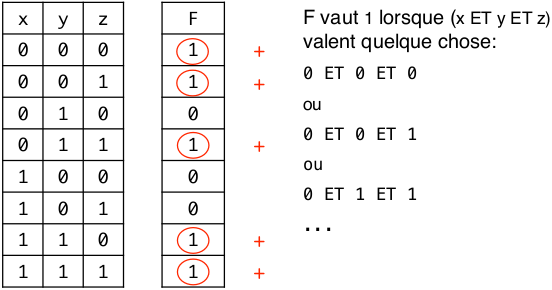
\includegraphics[scale=0.6]{ch2/image6}
\end{figure}
Pour écrire sous forme SdP, il suffit de prendre toutes les lignes où $F=1$, de réunir les variables d'une même ligne par $\cdot$ et joindre chaque colonne par $+$ en transformant les variables de cette manière :
\begin{itemize}
	\item $a$ si $a=1$
	\item $a'$ si $a=0$
\end{itemize}
Ainsi, la SdP est :
\begin{equation}
	F=x'\cdot y'\cdot z'+x\cdot' y'\cdot z+x'\cdot y\cdot z+x\cdot y\cdot z'+x\cdot y\cdot z
\end{equation}
\subsubsection{Table de Vérité vers PdS}
\label{subsubsec : TdV->PdS}
\begin{figure}[H]
	\centering
	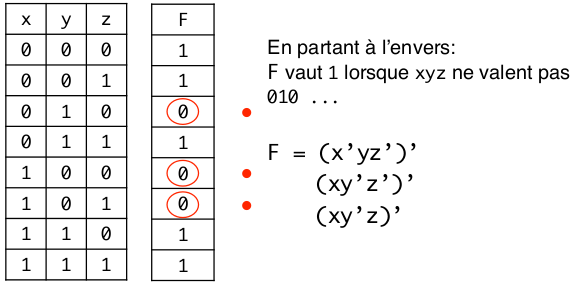
\includegraphics[scale=0.6]{ch2/image7}
\end{figure}
Pour écrire sous forme PdS, il suffit de prendre toutes les lignes où $F=0$, de réunir les variables d'une même ligne par $+$ et joindre chaque colonne par $\cdot$ en transformant les variables de cette manière :
\begin{itemize}
	\item $a$ si $a=0$
	\item $a'$ si $a=1$
\end{itemize}
Ainsi, la PdS est :
\begin{equation}
F=(x+y'+z)\cdot(x'+y+z)\cdot(x'+y+z')
\end{equation}
\begin{center}
	\textbf{OU BIEN}
\end{center}
On peut aussi faire la SdP pour $F=0$ (en gardant bien les conventions pour $SdP$) et noté $F'$ au lieu de $F$ et ensuite faire De Morgan ($(F')'=F$)
\begin{equation}
F'= x'\cdot y\cdot z'+x\cdot y'\cdot z'+x\cdot y\cdot z
\end{equation}
\begin{align}
	F &=(F')'=(x'\cdot y\cdot z')'\cdot(x\cdot y'\cdot z')'\cdot(x\cdot y\cdot z)'\\
	&= (x+y'+z)\cdot(x'+y+z)\cdot(x'+y+z')
\end{align}
\subsubsection{Schématique (logigrammes)}
Voici les différents symboles pour les opérateurs :
\begin{figure}[H]
	\centering
	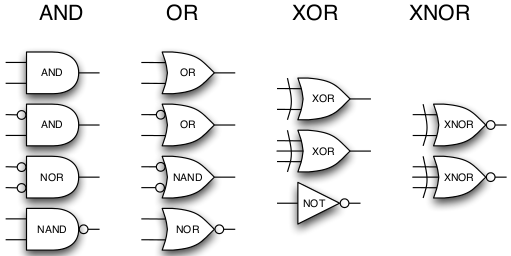
\includegraphics[scale=0.6]{ch2/image8}
\end{figure}
Dans un circuit en forme de SdP, on finit par une porte OU
\begin{figure}[H]
	\centering
	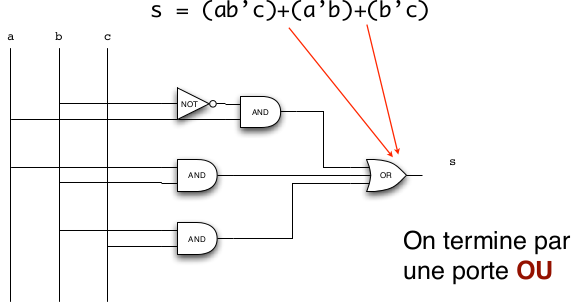
\includegraphics[scale=0.6]{ch2/image9}
\end{figure}
Dans un circuit en forme de PdS, on finit par une porte ET
\begin{figure}[H]
	\centering
	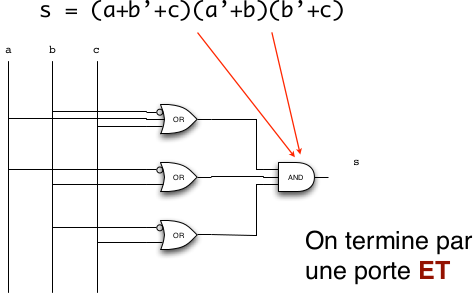
\includegraphics[scale=0.6]{ch2/image10}
\end{figure}
\section{Réalisation matérielle}
Chez soi (à partir du slide 50 cours 2).